\chapter{Stand der Technik}
\begin{onehalfspace}  
    \label{sec:theorie/standdertechnik}
        In diesem Kapitel wird der Stand der Technik näher beleuchtet. Der Fokus liegt dabei auf den Themen Daten, \ac{KI} und Bias. Zu Beginn wird auf basis der Literatur erläutert, was Daten sind, was Datenqualität bedeutet und worum es sich bei einem Bias handelt. Daraufhin wird näher auf \ac{KI}, das Teilgebiet \ac{ML} und die Ethik in der \ac{KI} eingegangen. Zuletzt werden die Themen in einen gemeinsamen Kontext gebracht und der Einfluss eines Bias auf eine \ac{KI} betrachtet sowie Gegenmaßnahmen untersucht. 
    
    \section{Daten als wertschöpfende Ressource}
    \label{subsec:datenchapter}
    \subsection{Daten}
    \label{subsubsec:daten}
        Dass Daten eine wertvolle Ressource seien, meinte bereits 2006 der britische Mathematiker Clive Humby mit dem berühmten Zitat: \glqq{}Data is the new oil\grqq{}.\cite{Frorbes2021} Hiermit ist gemeint, dass Daten in ihre Rohform nicht sonderlich wertvoll sind, diese jedoch an Wert gewinnen, sobald man beginnt sie zu verarbeiten. Denn lange Zeit waren Daten nur ein Nebenprodukt der Digitalisierung. Daten wurde gesammelt und gespeichert, aber nicht weiter verwendet. Mit dem technologischen Fortschritt im Bereich von Datenanalysen und mit aufkommen der \ac{KI} wurden Daten von Zeit zu Zeit immer wertvoller. So wurden neue Datengetriebene Geschäftsfeld ermöglicht, die einen Mehrwert aus Rohdaten schaffen können. Insbesondere das rasante Aufkommen des Internet of Things hat diese Entwicklung stark vorangetrieben. Seither steigt die Menge der jährlich gesammelten Daten exponentiell an.\cite{Otto2019}
        \\
        \begin{figure}[h]
            \centering
            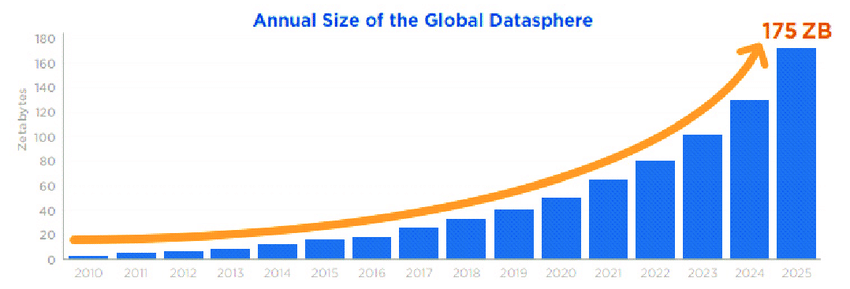
\includegraphics[width = 15.5cm]{Bilder/Annual_Data_Size.png}
            \caption{Weltweit jährlich anfallende Datenmenge \cite{Reinsel2018}}
            \label{fig:DataSize}
        \end{figure}
        \\
        Abbildung \ref{fig:DataSize} stammt aus dem Jahr 2018 und verdeutlicht, dass bereits damals erwartet wurde, dass bis im Jahr 2025 rund 175 Zetabyte Daten jährlich gesammelt werden. Im Vergleich dazu waren es 2018 gerade einmal 33 Zetabyte weltweit.\cite{Reinsel2018}\cite{Taleb2018}
        \\
        Der Begriff Daten selbst wird im ISO2382-1 Standard wie folgt definiert: \glqq{}reinterpretierbare Darstellung von Informationen in einer formalisierten Weise, die für die Kommunikation, Interpretation oder Verarbeitung geeignet ist\grqq{}.\cite{ISO2382} Daraus lässt sich ableite, dass Daten Informationen der Vergangenheit repräsentieren und für zukünftige Verwendung die Informationen aus der Vergangenheit in einer einheitlichen Form repräsentieren. Damit ist jedoch nicht die einheitliche Form der Daten selbst gemeint. 
        \\
        Daten gibt es in unterschiedlichen Formen. Es wird zwischen strukturierten und unstrukturierten Daten unterschieden. Strukturierte Daten sind Datensätze bestehend aus einzelnen Variablen die eindeutige Größen Darstellen. Beispiel hierfür sind Sensordaten oder Unternehmenszahlen aus einem ERP System. Sie werden tabbelarisch gespeichert und können einfach weiter verarbeitet werden. Oftmals sind diese Daten heterogen, was bedeutet, dass sich die Variablen unterscheiden und bspw. Spalte 1 vollkommen andere Daten behinhaltet als Splate 2. Ein Beispiel hierfür wären Sensoren für Luftfeuchtigkeit und Helligkeit in einem Büro. Als unstrukturierte Daten bezeichnet man Daten, die nicht in sinnvolle einheitliche Variablen unterteilt werden können. Zu dieser Art von Daten zählt man Bilder, Videos, Audio und Textdaten. Sie sind meist homogen, denn die Pixel in einem Bild nehmen zwar unterschiedliche RGB Werte an, jedoch repräsentieren sie alle einen Pixel. Dabei ist es egal ob es sich um Pixel 1 oder Pixel 42 handelt.\cite{Horn2022} Bei dieser unvorstellbar großen Datenmenge die jährlich generiert wird, wird davon ausgegangen, dass rund 80\% als unstrukturierte Daten vorliegen.\cite{Otto2019}
        \\
        Häufig wird in dem Zusammenhang mit Daten auch von Big Data gesprochen. Eine einheitliche Definition für den Begriff Big Data existiert jedoch nicht. Denn der Begriff Big Data umfasst die gesamte Wertschöpfungskette. Diese beinhaltet die Datenerzeugung, das Sammel und Speichern der Daten bis hin zur Verarbeitung und Nutzung für Analysen oder Visualisierungen.\cite{Taleb2018}\cite{Faroukhi2020} Es handelt sich dabei um Informationen mit hohem Volumen (high-volume), hoher Geschwindigkeit (high-velocity) und hoher Vielfalt(high-variety). Diese drei charakteristischen Eigenschaften werden in der Literatur auch als die \glqq{}3 V rule\grqq{} bezeichnet und ist in den meisten Definitionen wiederfinden.\cite{Taleb2018}\cite{Yalaoui2021} 
        \begin{figure}[h]
            \centering
            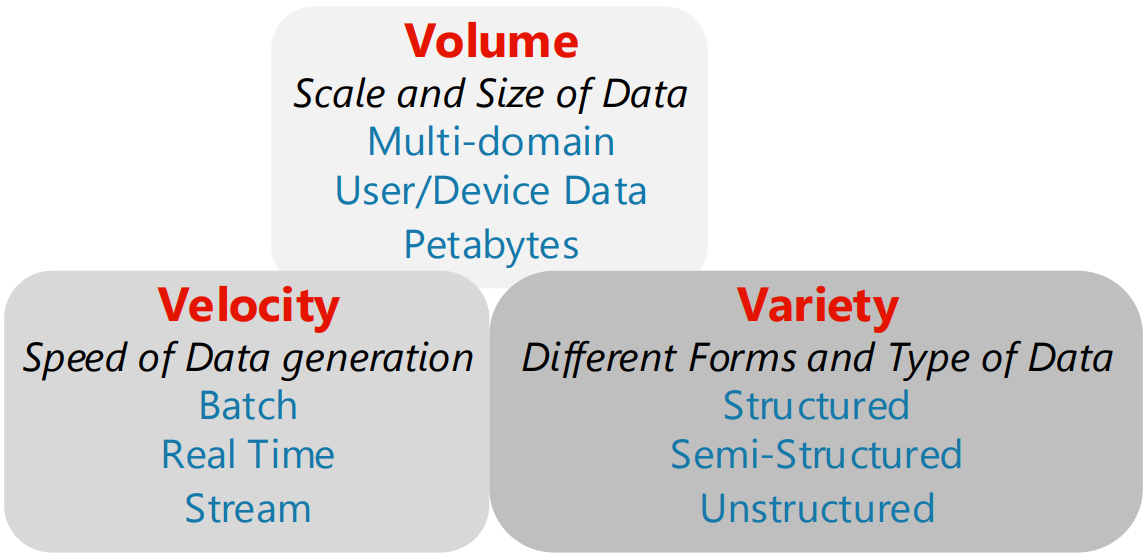
\includegraphics[width = 6.7cm]{Bilder/3VRule.png}
            \caption{Big Data 3 V rule \cite{Taleb2018}}
            \label{fig:3VRule}
        \end{figure}
        \\
        In der Abbildung \ref*{fig:3VRule} werden diese Eigenschaften die Big Data mit sich bringt näher beschrieben. Unter \glqq{}Volume\grqq{} wird die große Menge an Daten, also der damit verbundene benötigte Speicher, und ihre Skalierbarkeit betrachtet. Bei der \glqq{}Velocity\grqq{} liegt der Fokus auf der Geschwindigkeit in der die Daten erzeugt werden. Dies hat wiederrum je nach Geschwindigkeit der Datenerzeugung einfluss auf das Volumen. Abschließend in dem Dreieck gibt es die \glqq{}Variety\grqq{}. Big Data ist von natur aus eine Vielfalt an strukturierten und unstrukturierten Daten. All diese drei Eigenschaften beeinflussen sich gegenseitig und bilden die grundlegenden Eigenschaften von Big Data.
        \\
        In Rohform sind diese Daten, wie eingangs erwähnt, jedoch nicht sonderlich von Wert. Egal ob Big Data oder nicht, einen Mehrwert und Infromationen liefern sie erst, sobald man sie nutzt. Dabei ist es egal ob für Simulationen, Monitoring oder \ac{KI}. In der Vergangenheit sind Daten ein Nebenprodukt der Digitalisierung gewesen. Heute sind sie ein eigenes Geschäftsfeld und \glqq{}Enabler\grqq{} für viele bisher nicht möglich gewesenen Anwendungen.\cite{Otto2019}\cite{Gröger2021}

    \subsection{Datenqualität}
    \label{subsubsec:datenqualität}
        Im Zusammenhang mit Daten fällt immer häufiger auch der Begriff Datenqualität. Hier trifft Quantität auf Qualität. Wie bereits erwähnt, ist die Menge an Daten die bereits zur Verfügung steht, rießig. Quantität ist daher nicht das Problem. Die Qualität der Daten hat hier jedoch sehr großen Einfluss. Nicht selten können Daten nicht verwendet werden, da die Qualität nicht ausreichend ist. Gerade für Analysen, Auswertungen und Vorhersagen, wie sie durch die \ac*{KI} getroffen werden sollen, wird hohe Datenqualität benötigt.\cite{Byabazaire2020}
        \\
        Datenqualität selbst lässt sich auf unterschiedliche Arten und Weisen verstehen.\cite{Yalaoui2021} Eine gängige Definition für Datenqualität in der Literatur ist:\glqq{}fitness for use\grqq{}.\cite{Faroukhi2020} Es bedeutet, dass die Datenqualität von Nutzungskontext und Anwendungsfall abhängt und in erster Linie nicht allgemeine Qualitätsanforderungen erfüllt werden, sondern die für den Use Case benötigten Qualitätsanfoderungen.\cite{Faroukhi2020}\cite{Yalaoui2021}
        \begin{figure}[h]
            \centering
            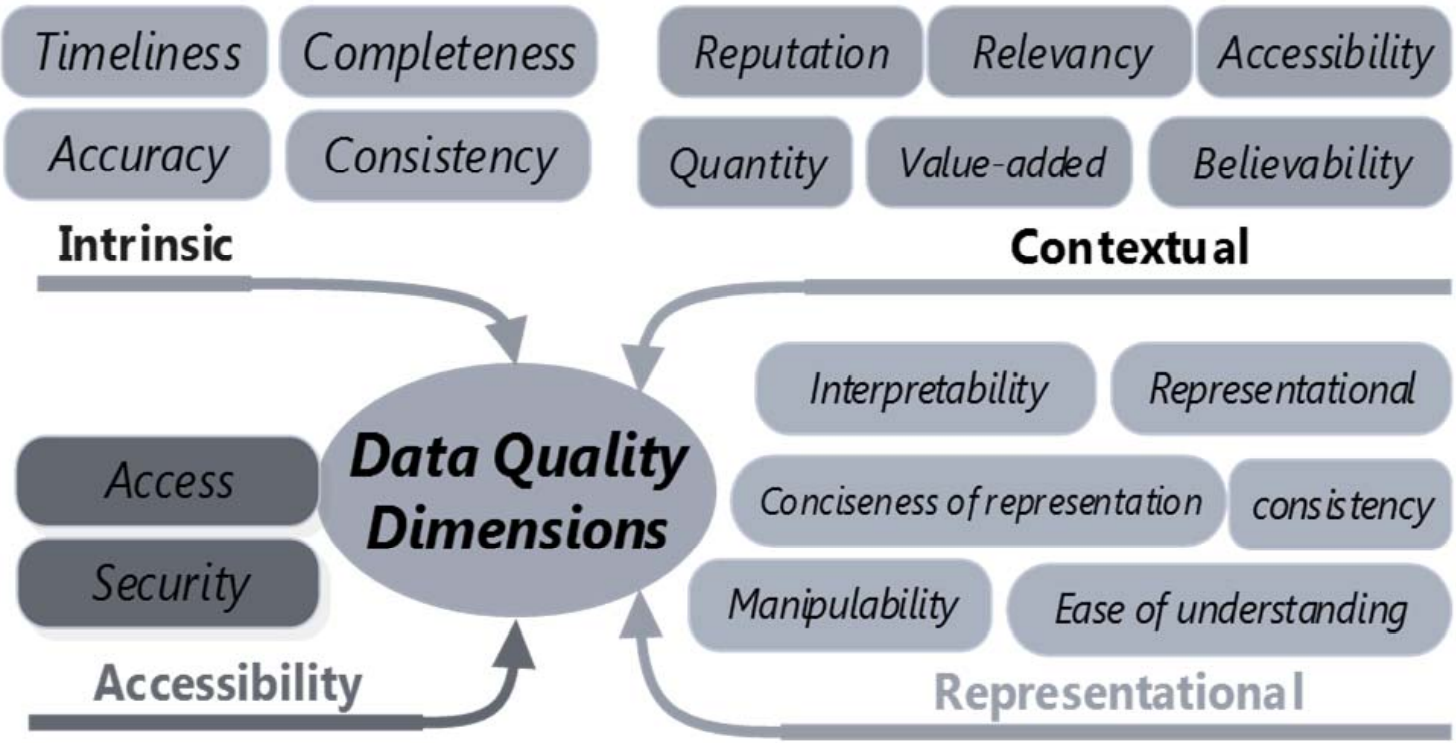
\includegraphics[width = 9cm]{Bilder/Data_quality_dimensions.png}
            \caption{Data Quality Dimensions \cite{Taleb2018}}
            \label{fig:DataQualityDimensions}
        \end{figure}
        \\
        Für die Validierung der Datenqualität gibt es die sogenannten Data Quality Dimensions. In Abbildung \ref{fig:DataQualityDimensions} sind die vier unterschiedlichen Dimensionen: Intrinsic (\ac{dt}.: Intrinsisch), Contextual (\ac{dt}.: Kontextbezogen), Accessibility (\ac{dt}.: Zugänglichkeit ) und Representational (\ac{dt}.: Repräsentativ) dargstellt. Jede Dimension besitzt eigene Merkmale an denen die Datenqualität gemessen werden kann. Näher erläutert werden die Dimensionen in der Tabelle \ref*{table:0}.
        \\
        \begin{table}[h]
            \centering
            \begin{adjustbox}{width=\textwidth}
            \resizebox{\textwidth}{!}{\begin{tabular}{|l|l|}
            \hline
            Intrinsic        & \begin{tabular}[c]{@{}l@{}}
                                    Zur intrinsischen Datenqualität gehören, wie in Abbildung \ref*{fig:DataQualityDimensions} zu sehen,\\
                                    die Merkmale: Zeitlos, Vollständigkeit, Genauigkeit, Konsistenz. Die \\
                                    intrinsische Dimension bildet die Qualitätsmerkmale der Daten selbst ab. \\
                                    und gibt Aufschluss über Objektivität und Glaubwürdigkeit der Daten.\cite{Yalaoui2021}
                                \end{tabular}  \\ \hline
            Contextual      &   \begin{tabular}[c]{@{}l@{}}
                                    Bei der kontextbezogenen Datenqualität wird betrachtet in welchem Ausmaß \\
                                    die Daten für den Nutzenden einsetzbar sind. Darin werden Eigenschaften wie:\\
                                    Datenmenge (Quantität), Zugänglichkeit, Aktualität und Mehrwert \\
                                    der Daten betrachtet um die Nutzbarkeit zu messen.\cite{Otto2019}
                                \end{tabular}  \\ \hline
            Representational &  \begin{tabular}[c]{@{}l@{}}
                                    Repräsentativ bedeutet im Kontext der Datenqualität, dass die Daten \\
                                    Interpretierbarkeit und dabei primär einfach zu Verstehen sind, \\
                                    Konsistaent sind und  Manipulierbarkeit, also Veränderbar sind.\cite{Byabazaire2020}

                                \end{tabular}  \\ \hline
            Accessibility    &  \begin{tabular}[c]{@{}l@{}}
                                    Die vierte Dimension, die Zugänglichkeit, bezieht sich Insbesondere \\
                                    auf das Speichersystem der Daten. Diese Dimension wird an der möglichst\\
                                    einfachen Zugänglichkeit und der entgegenstehenden Sicherheit der \\
                                    Daten gemessen.\cite{Byabazaire2020}
                                \end{tabular}  \\ \hline           
            \end{tabular}}
            \end{adjustbox}
            \caption{Data Quality Dimensions Merkmale}
            \label{table:0}
        \end{table}
        \\
        Datenqualität lässt sich in unterschiedlichsten Dimensionen und anhand unterschiedlicher Qualitätsmerkmale messen. Die in Abbildung \ref*{fig:DataQualityDimensions} dargestellten und in Tabelle \ref*{table:0} erläuterten Dimensionen sind dabei nur eine der gängigen Modelle aus der Literatur. 
        \\
        Trotz des Bewusstseins für Datenqualität, besteht rund 80 Prozent der Arbeit eines Data Scientist daraus, Daten aufgrund von Qualitätsanfoderungen vorzuverarbeiten.\cite{Horn2022} Angefangen beim einfachen Umwandeln bis hin zu komplexeren Bereinigungen und Encodierungen der Daten. Daten werden in den meisten Fällen nicht die gewünschten Qualitätsanforderungen erfüllen können. Datenqualität ist keine verallgemeinerbare Formel, sondern immer abhängig vom Anwendungsfall und dem Kontext in dem die Daten genutzt werden sollen.
        \\
        Dass Datenqualität eine wichtige Rolle spielt, unabhängig von dem Verwendungszweck, ist keine Frage. In der Wissenschaft sowie Wirtschaft wird sich immer intensiver mit der Themaitik der Datenqualität auseinandergesetzte, da heutzutage die Quantität kam noch ein Problem darstellt, sondern viel mehr die Qualität der Daten.\cite{Lis2019} Denn Quantität ist nicht gleich Qualität!

%#########################################

    \newpage
    \section{Künstliche Intelligenz}
    \label{subsec:KIandML}
    \subsection{Künstliche Intelligenz Allgemein}
    \label{subsubsec:KIAllgemein}
        \ac{KI} als Begriff wird vielseitig und unterschiedlich Verwendet. Die Vision von \ac{KI} ist es, die intellektuellen und menschlichen Fähigkeiten als ein KI-System nachzubilden.\cite{Lis2019} Letztendlich beschreibt \ac{KI} ein Forschungsbreich aus der Informatik, der aus einer Vielzahl aus Technologien besteht.\cite{HEGKI2019Definition} 
        \begin{figure}[h]
            \centering
            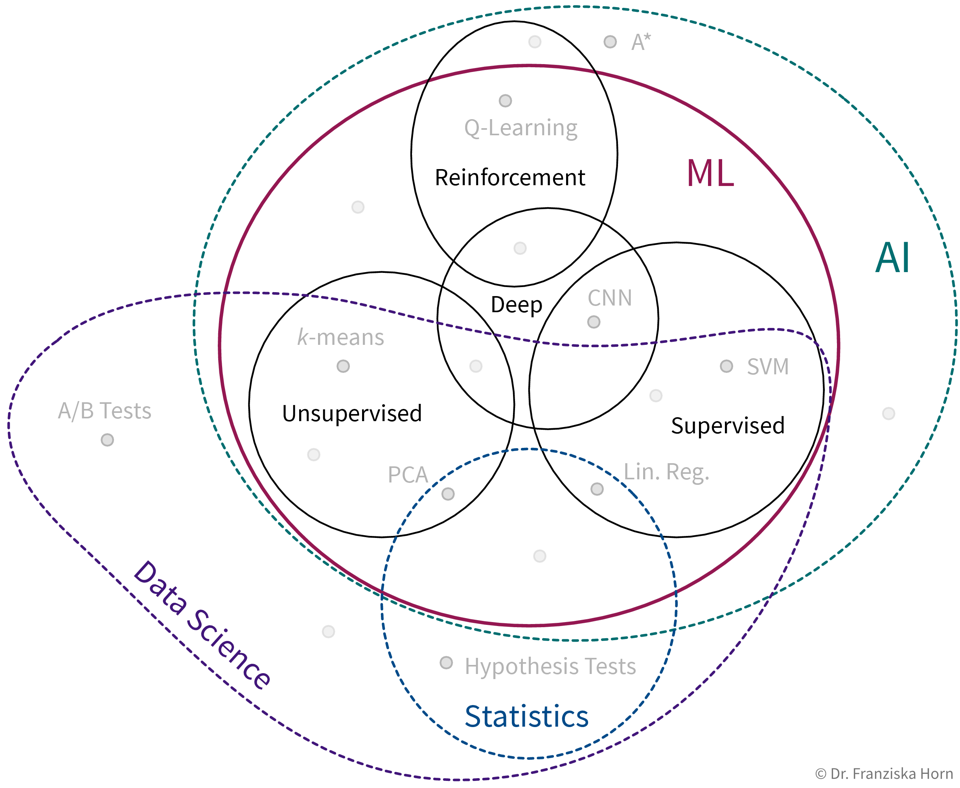
\includegraphics[width = \textwidth]{Bilder/ml_toolset.png}
            \caption{Exemplarisch dargestellte Disziplinen von \ac{KI}\cite{Horn2022}}
            \label{fig:ml_toolset}
        \end{figure}
        \\
        Die Abbildung \ref*{fig:ml_toolset} ziegt exemplarisch, welche Position \ac*{KI} in der Infromatik einnimmt. Zur \ac{KI} gehören bekannte Teilgebiet wie das \ac*{ML}, Optimierungsalgorithmen, aber auch  in der Robotik kommt \ac{KI} zum Einsatz. Selbst wird die Disziplin aber auch von anderen übergeordneten Disziplinen genutzt.\cite{HEGKI2019Definition} Ein Beispiel hierfür ist Data Science. Die Abbildung \ref*{fig:ml_toolset} veranschaulticht, dass einige Aspekte aus der \ac{KI} im Bereich Data Science augegriffen werden, jedoch deutlich mehr als nur \ac{KI} hinter Data Science steckt.
        \\
        In der Literatur wurde in der Vergangenheit oft zwischen \glqq{}schwacher\grqq{} und \glqq{}starker\grqq{} \ac{KI} unterschieden. Eine schwache \ac{KI} ist dabei für ein spezifisches Anwendungsproblem konzipiert. Der \ac{KI} wird eine Aufgabe gegeben und diese versucht mittels Algorithmen und mathematischen Funktionen die Aufgabe zu lösen. Diese Art der \ac{KI} versucht Aufgaben zu lösen und Ergebnisse zu liefern, wie sie durch menschliche Intelligenz entstehen können.\cite{Lis2019} Ein Beispiel hierfür ist die Bilderkennung, bei der Entschieden wird, ob auf dem Bild eine Erdbeere zu sehen ist, oder nicht.
        \\
        Als starke \ac{KI} wird ein System verstanden, welches in der Lage ist ein breites Spektrum an Aufgaben zu erledigen.\cite{Datenkommission2019} Sie verfügt über weitere Methoden zur Datenverarbeitung. In dieser Form der \ac{KI} wird mehr versucht die menschlichen Fähigkeiten und Intelligenz abzubilden. Es wird nicht nach eine spezifischen Vorgehensweise vorgegangen, sondern Aufgaben werden mit individuellen Lösungenswegen erledigt.\cite{Lis2019}
        \\
        Mit dem Begriff \ac{KI} wird demzufolge nur ein grundlegendes Prinzip von \ac*{KI}-Systemen definiert. Die Aufgabe dieser \ac*{KI}-Systeme ist es, Daten jeglicher Form zu interpretieren, Schlussfolgerungen daraus zu ziehen und eine Aussage über das zu erreichende Ziel zu liefern. Unabhängig davon, ob es sich um einen optimalen Lösungsweg, eine Vorhersage oder eine Schlussfolgerung handelt. \cite{HEGKI2019Definition}    
    
    \subsection{Teilgebiet maschinelles Lernen}
    \label{subsubsec:teilgebietML}
        Maschinelles Lernen ist das bekannteste Teilgebiet der \ac{KI}. Unter \ac{ML} wird verstanden, 
        \\
        Um das Teilgebiet \ac{ML} detaillierter zu betrachten, unterscheidet man zwischen \glqq{}superviced learning\grqq{}(\ac*{dt}.: überwachtes Lernen), \glqq{}unsuperviced learning\grqq{}(\ac*{dt}.: unüberwachtes Lernen) und dem \glqq{}reinforcement learning\grqq{}(\ac*{dt}.: bestärktes Lernen).\cite{Horn2022}\cite{Datenkommission2019} Bei dieser Unterschiedung wird zwischen der Art des Lernens unterschieden. 
        \\
        \begin{figure}[h]
            \centering
            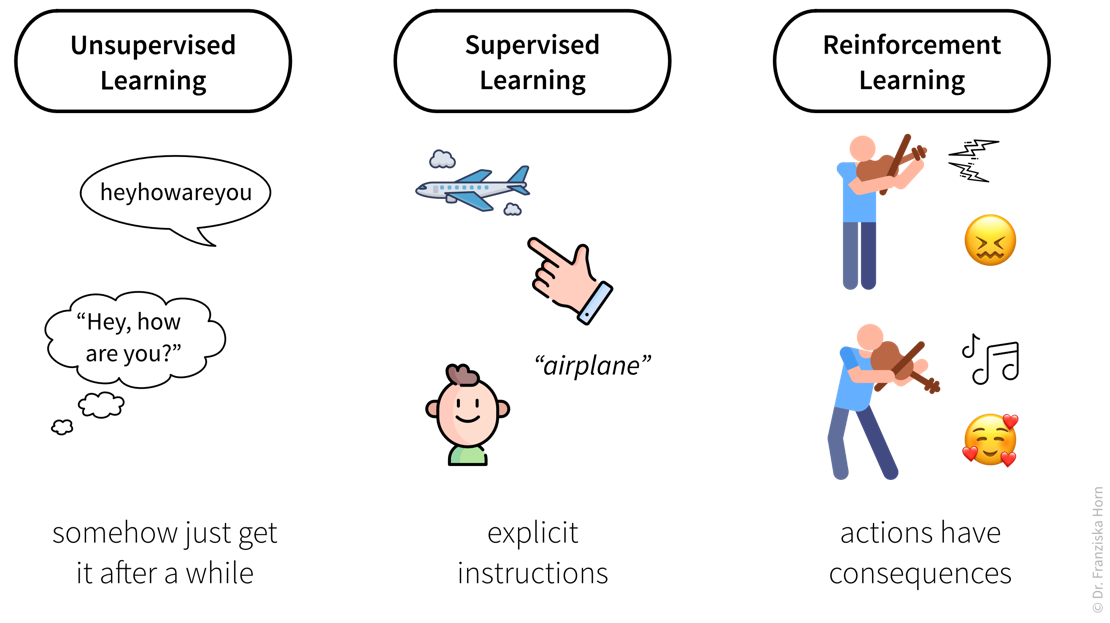
\includegraphics[width = 12cm]{Bilder/ml_algorithms.png}
            \caption{Arten des maschinellen Lernen\cite{Horn2022}}
            \label{fig:ml_algorithms}
        \end{figure}
        \\
        Die Abbildung \ref*{fig:ml_algorithms} stellt diese unterschiedlichen Arten des Lernens vereinfacht dar. Das unsuperviced learning funktioniert, indem ich wie in Abbildung \ref*{fig:ml_algorithms} einen Text ohne zusätzliche Informationen angebe, und das Modell selbstständig den Zusammenhang erkennt und die Frage identifiziert. Diese Art ist vergleichbar mit dem menschlichen Lernen durch Ausprobieren. 
        Das überwachte Lernen, ist die natürliche Form der menschlichen Wissensaneignung. Hier wird dem Modell etwas beigebracht. Das Beispiel der Abbildung \ref*{fig:ml_algorithms} veranschaulicht es sehr gut. Hier wird auf ein Flugzeug gezeigt und dem Kinde gesagt, dass es sich um ein Flugzeug handelt. Das Kind merkt sich dies und ist beim nächsten mal selbst in der Lage das Flugzeug zu erkennen. In stark vereinfachter Form gilt dies auch für ein Modell, dem Modell wird beigebracht, dass es sich um ein Flugzeug handelt und dieses lernt die Assoziation eines Flugzeugs mit dem Begriff Flugzeug.
        Die dritte und bisher noch nicht sehr weit verbreite Art des Lernens ist das bestärkte Lernen. Es handelt sich dabei um ein Feedback basiertes Lernen. Das bedeutet, dass das Modell frei Handeln und Entscheiden darf. Die Handlungen werden jedoch danach bewertet und das Modell bekommt gesagt, ob es gut war oder nicht. Das Beispeil mit dem Geigenspieler der zuerst spielt und im nachhinein Feedback bekommt aus Abbildung \ref*{fig:ml_algorithms} illustriert die Form des Lernens recht passend. 
        \\
        Im Rahmen dieser Arbeit wird sich speziell auf das superviced Learning fokussiert. Superviced learning wird immer dann eingesetzt, wenn man etwas auf Basis von Eingabedaten vorhersagen, Schlussfolgern oder Entscheiden möchte. Die bekannten Beispiele sind hier die Bildererkennung von Google mit der Unterscheidung von Hunden und Katzen. 
        \\
        Es gibt aber auch einige Risiken, die im Zusammenhangmit \ac{ML} auftreten. Für das beschriebene Lernverfahren des superviced learning ist es zum einen wichtig eine ausreichende Datenmenge zu besitzen. 
        Des weiteren muss beim Trainieren und Lernen des Modells das Modell selbst bewertet werden. Dazu gibt es unterschiedliche Metriken die es einem ermöglichen die Qualität eines Modells zu bewerten. Denn wird dies nicht getan, kann es passieren, dass das Modell over- oder underfitted. 
        \\
        ZU ÜBERARBEITEN\cite{Döbel2018}\cite{Ng2018}
        \\

    \subsection{Ethik in der künstlichen Intelligenz}
    \label{subsubsec:ethikinderKI}
        Spacer
        \\
        \begin{figure}[h]
            \centering
            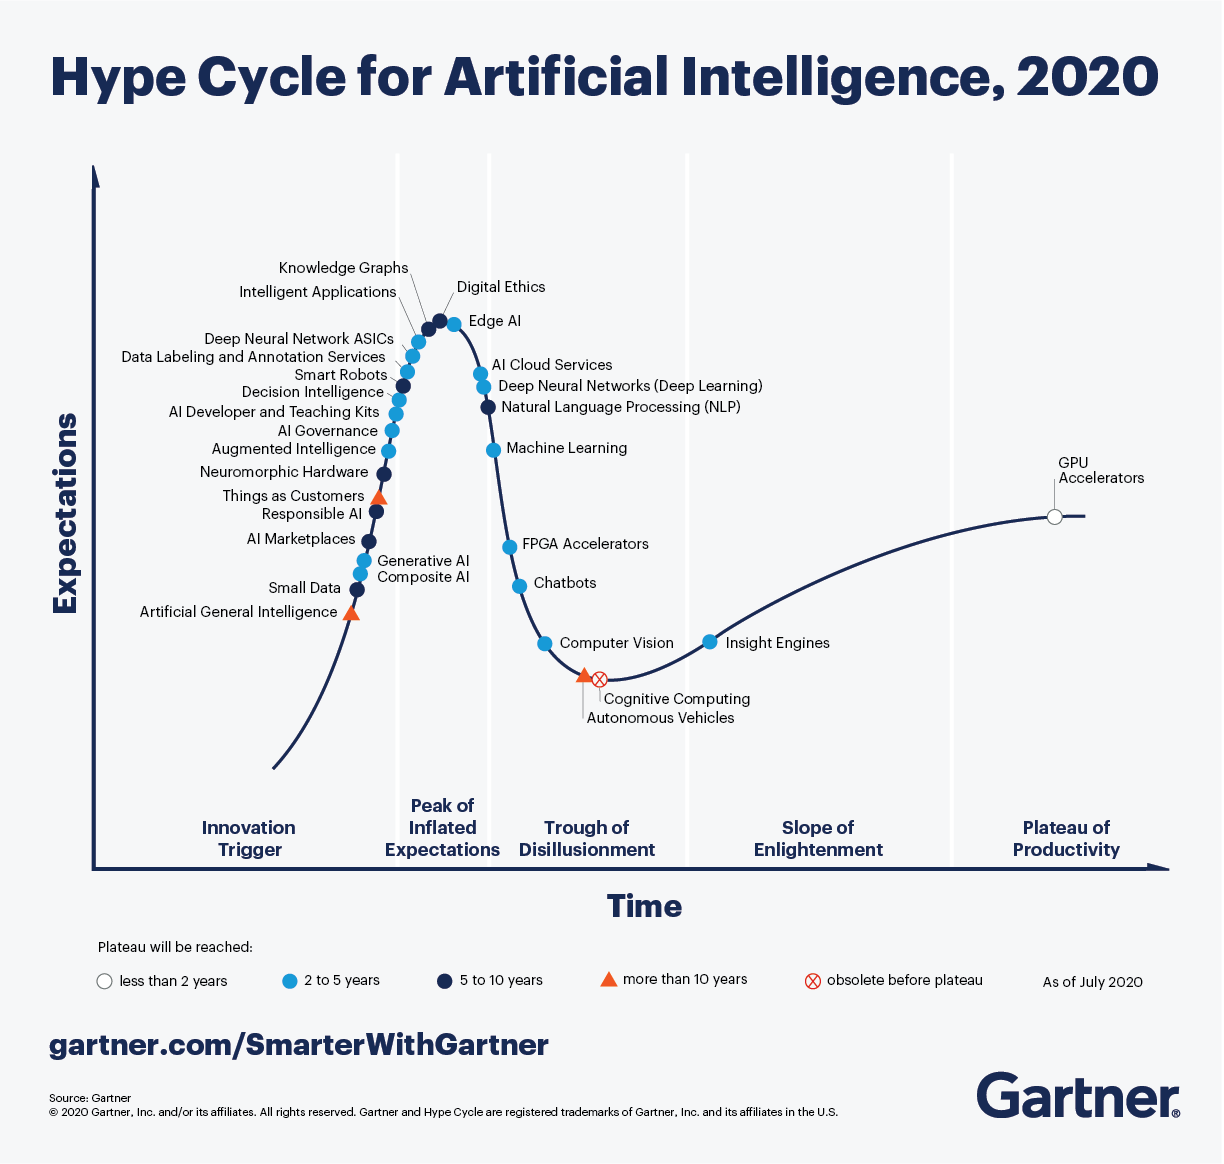
\includegraphics[width = \textwidth]{Bilder/Gartner_hypeCycle.png}
            \caption{Gartner Hype Cycle für \ac*{KI}\cite{Goasduff2020}}
            \label{fig:HypeCycle}
        \end{figure}
        \\
        - Ethik spielt eine große Rolle in der Gesellschaft
        - EU Setzt sich mit Richtlinien auseinandern
        - Diskriminierung durch KI ist ein fatales Problem
        - Maschinen besitzen keine Moral und Ethisches werteverständnis
        \cite{Cremers2019} \cite{Beckert2021} \cite{Hallensleben2020} \cite{HEGKI2019}

%#########################################

    \newpage
    \section{Bias im Zusammenhang mit \ac{KI}}
    \label{subsec:KIundbias}
    \subsection{Bias}
    \label{subsubsec:Bias}
        - ML ist immer auf Basis von Daten aus der Vergangenheit 
        -   Begriffserklärung: Data Bias vs Bias Verzerrung\\
        -   Arten von Bias: \\
            -   Bias durch Abwesenheit - Wenn eine Info fehlt, kann das zu Diskriminierung führen. \\
            -   Diskriminierung durch Menschen. \\
        Arten von Bias: Cognitive, Social, Perceptual und Motivational Bias \cite{HEGKI2019Definition}\cite{Parkavi2018}

    \subsection{Diskriminierung durch Bias in Daten}
    \label{subsubsec:diskriminierungdurchverzerrung}
        - Bias in Daten
        - Wie funktioniert Bias in Daten
        - Was ist die Problematik
        - Welche Auswirkungen hat es 
        - Realbeispiele <-- Bewerbungsverfahren
        \cite{IncidentDatabase2015}

    \subsection{Gegenma{\ss}nahmen}
    \label{subsubsec:gegenmassnahmen}
        - Was kann man dagegen tun?
        - Gibt es möglichkeiten Trainingsdaten künstlich zu erzeugen und so eine neutrale betrachtung zu schaffen
        - Parameter entfernen als Lösung --> Die KI wird aber dadurch schlechter 
        - 

        Wenn der Parameter mit dem Bias entfernt wird, wird das Ergebnis erstmal schlechter. 
        
    \newpage
\end{onehalfspace}